\documentclass[a4paper]{article}

% --- Packages ---

\usepackage{a4wide}
\usepackage[utf8]{inputenc}
\usepackage{amsmath}
\usepackage{mathtools}
\usepackage{amssymb}
\usepackage[english]{babel}
\usepackage{mdframed}
\usepackage{systeme,}
\usepackage{lipsum}
\usepackage{relsize}
\usepackage{caption}
\usepackage{tikz}
\usepackage{tikz-3dplot}
\usetikzlibrary{shapes.geometric}
\usepackage{pgfplots}
\usepackage{pgfplotstable}
\pgfplotsset{compat=newest}%1.7}
\usepackage{harpoon}%
\usepackage{graphicx}
\usepackage{wrapfig}
\usepackage{subcaption}
\usepackage{authblk}
\usepackage{float}
\usepackage{listings}
\usepackage{xcolor}
\usepackage{chngcntr}
\usepackage{amsthm}
\usepackage{comment}
\usepackage{commath}
\usepackage{hyperref}%Might remove, adds link to each reference
\usepackage{url}
\usepackage{calligra}
\usepackage{tikz}
\usepackage{pgf}

% --- Bibtex ---

%\usepackage[backend = biblar,]{bibtex}

%\addbibliografy(ref.bib)

% --- Commands --- 

\newcommand{\w}{\omega}
\newcommand{\trace}{\text{Tr}}
\newcommand{\grad}{\mathbf{\nabla}}
%\newcommand{\crr}{\mathfrak{r}}
\newcommand{\laplace}{\nabla^2}
\newcommand{\newparagraph}{\vspace{.5cm}\noindent}

% --- Math character commands ---

\newcommand{\curl}[1]{\mathbf{\nabla}\times \mathbf{#1}}
\newcommand{\dive}[1]{\mathbf{\nabla}\cdot \mathbf{#1}}
\newcommand{\res}[2]{\text{Res}(#1,#2)}
\newcommand{\fpartial}[2]{\frac{\partial #1}{\partial #2}}
\newcommand{\rot}[3]{\begin{vmatrix}\hat{x}&\hat{y}&\hat{z}\\\partial_x&\partial_y&\partial_z\\#1&#2&#3 \end{vmatrix}}
\newcommand{\average}[1]{\langle #1 \rangle}
\newcommand{\ket}[1]{|#1\rangle}
\newcommand{\bra}[1]{\langle #1|}


%  --- Special character commands ---

\DeclareMathAlphabet{\mathcalligra}{T1}{calligra}{m}{n}
\DeclareFontShape{T1}{calligra}{m}{n}{<->s*[2.2]callig15}{}
\newcommand{\crr}{\mathcalligra{r}\,}
\newcommand{\boldscriptr}{\pmb{\mathcalligra{r}}\,}


\title{Handin 2 : FK8202}
\author{Author : Andreas Evensen}
\date{Date: \today}

% --- Code ---

\definecolor{codegreen}{rgb}{0,0.6,0}
\definecolor{codegray}{rgb}{0.5,0.5,0.5}
\definecolor{codepurple}{rgb}{0.58,0,0.82}
\definecolor{backcolour}{rgb}{0.95,0.95,0.92}

\lstdefinestyle{mystyle}{
    backgroundcolor=\color{backcolour},   
    commentstyle=\color{codegreen},
    keywordstyle=\color{magenta},
    numberstyle=\tiny\color{codegray},
    stringstyle=\color{codepurple},
    basicstyle=\ttfamily\footnotesize,
    breakatwhitespace=false,         
    breaklines=true,                 
    captionpos=b,                    
    keepspaces=true,                 
    numbers=left,                    
    numbersep=5pt,                  
    showspaces=false,                
    showstringspaces=false,
    showtabs=false,                  
    tabsize=2
}

\lstset{style=mystyle}

\begin{document}

\maketitle

\section{Questions}
Suppose a gas in 2 dimension consisting out of $N$ particles. The model has periodic boundary conditions, and the particles can either interact with each other with {\color{red}a Lennard-Jones potential} or {\color{blue}as hard spheres}.
\begin{figure}[H]
    \centering
    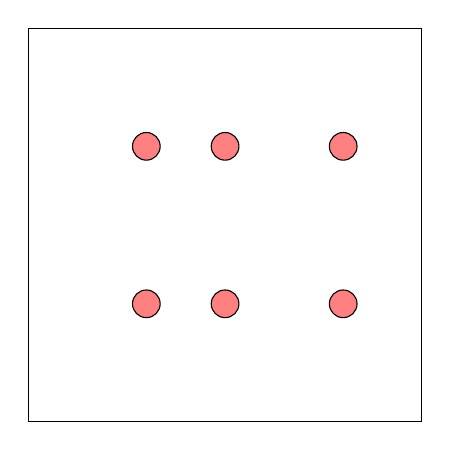
\begin{tikzpicture}[scale = 0.5]
        \draw (0,0) rectangle (10,10);
        \foreach \x in {3,5,8}{
            \foreach \y in {3,7}{
               \draw[fill = red!50] (\x,\y) circle (10 pt); 
            };
        };
    \end{tikzpicture}
\end{figure}
\subsection*{1.a}
Suggest and motivate how to solve the equations of motion for the particles when they interact with each other with a {\color{red} Lennard-Jones potential}.

\newparagraph
\textbf{Answer:} In order to solve the equations of motion for particles when interacting with a potential, one has to solve the equations of motion for each particle. The equations of motion for a particle $i$ is given by Newton's second law,
\begin{equation*}
    m_i\ddot{\mathbf{r}}_i = \mathbf{F}_i,
\end{equation*}and the force $\mathbf{F}_i$ is given by the gradient of the potential energy $\mathcal{V}(\mathbf{r}_i, \{\mathbf{r}_j\})$,
\begin{align*}
    \mathcal{V}(\mathbf{r_i}, \{\mathbf{r}_j\}) &= \sum_{j\neq i} \epsilon\left[\left(\frac{\sigma}{\abs{\mathbf{r}_i - \mathbf{r}_j}}\right)^{12} - \left(\frac{\sigma}{\abs{\mathbf{r}_i - \mathbf{r}_j}}\right)^{6}\right].
\end{align*}From there, one can use the Verlet integration method to solve the equations of motion. The Verlet integration method is a numerical method for solving the equations of motion, which is symplectic and conserves energy. The Verlet integration method is given by the following algorithm,
\begin{align*}
    \mathbf{r}_i(t + \Delta t) &= \mathbf{r}_i(t) + \mathbf{v}_i(t)\Delta t + \frac{1}{2}\mathbf{a}_i(t)\Delta t^2,\\
    \mathbf{v}_i(t + \Delta t) &= \mathbf{v}_i(t) + \frac{1}{2}\left[\mathbf{a}_i(t) + \mathbf{a}_i(t + \Delta t)\right]\Delta t,
\end{align*}where $\mathbf{a}_i(t)$ is the acceleration of particle $i$ at time $t$. The acceleration is given by the force divided by the mass of the particle,

\subsection*{1.b}
Suggest and motivate how to solve the equations of motion for the particles when they interact with each other as {\color{blue} hard spheres}.

\newparagraph
\textbf{Answer:} When solving a hard sphere problem, one assumes that the atoms are free to move with some velocity, but that they collide. When colliding, one assumes an elastic collision, and that the particles bounce off each other.
In this case, the interaction between the atoms are purely elastic, and an interaction force, such as the force exerted by the Lennard-Jones potential, is not present.

\newparagraph
Thus, one computes the new position of the particles in the following manner:
\begin{align*}
    \mathbf{r}_i(t + dt_i) = \mathbf{r}_i(t) + \mathbf{v}_i(t)dt_i,
\end{align*}where $dt_i$ is the time-step for particle $i$ to collide with another particle, or the boundary. One then takes the minimum $dt_i$ for all particles, and updates the position of all particles with this time-step.
One computes $dt_i$ in the following manner, when approximating that the particles are spheres of radii $R$ and that the radii of the particles are the same:
\begin{align*}
    dt_i &= \sum_{j \neq i}\frac{1}{\abs{\dot{\mathbf{r}}_i - \dot{\mathbf{r}}_j}^2}\cdot\\
    &\left[-\left(\mathbf{r}_i - \mathbf{r}_j\right)\cdot\left(\dot{\mathbf{r}}_i - \dot{\mathbf{r}}_j\right)\pm\sqrt{\left[\left(\mathbf{r}_i - \mathbf{r}_j\right)\cdot\left(\dot{\mathbf{r}}_i - \dot{\mathbf{r}}_j\right)\right]^2 + \left(\dot{\mathbf{r}}_i - \dot{\mathbf{r}}_j\right)\left(4R^2 - \abs{\mathbf{r}_i - \mathbf{r}_j}\right)}\right].
\end{align*}In doing this, one has to be careful of particles that are close to the boarder, since they might bounce of each other as illustrated in the figure below.
\begin{figure}[H]
    \centering
    \begin{tikzpicture}
        \draw (-.5, 2.5) circle (15pt);
        \draw (0,0) -- (0, 5);
        \draw (+.5, 2.5) circle (15pt);
    \end{tikzpicture}
    \caption{Particles close to the boundary that are colliding.}
\end{figure}

\subsection*{2}
Describe in detail how the force is calculated for a given atom, say $i = 1$, at a particular configuration $\{r_i\}~ i = 1,N$ in the Lennard-Jones model. Notice, mention approximations that you introduce. 

\newparagraph
\textbf{Answer:} The force between to particles $i$ and $j$ exerted by the Lennard-Jones potential can be written as:
\begin{align*}
    \mathbf{F}_{i,j} &= -4\epsilon\left(12\cdot\left(\frac{\sigma}{\abs{\Delta\mathbf{r}_{i,j}}^2}\right)^{12} - 6\cdot\left(\frac{\sigma}{\abs{\Delta\mathbf{r}_{i,j}}^2}\right)^{6}\right)\frac{\Delta\mathbf{r}_{i,j}}{\abs{\Delta\mathbf{r}_{i,j}}^2}.
\end{align*}Here, $\Delta\mathbf{r}_{i,j}$ is the distance between closes neighboring atoms in each image; we approximate that the interaction is dominated by the closes pair in each image. Thus, we say that there exist $\rho\cdot N$ images in each image.Thus, the force exerted by a Lennard-Jones potential on particle $i$ form all other particles $j$ can be written as:
\begin{align*}
    \mathbf{F}_i &= \sum_{j\neq i}\mathbf{F}_{i,j}.
\end{align*}Hence, if $i = 1$ and one computes the sum of the forces exerted by all other particles, the expression reduces to:
\begin{align*}
    \mathbf{F}_1 &= \sum_{j = 2}^{N\cdot\rho}\mathbf{F}_{1,j}.
\end{align*}This has a time-complexity of $\mathcal{O}(N\cdot\rho)$ for finding the force exerted by all other particles on particle $1$.
\subsection*{3}
Describe in detail how different operations in the molecular dynamics algorithm of the hard sphere gas scales (both in terms of CPU time and CPU memory) with the number of atoms.

\newparagraph
\textbf{Answer:} In the beginning of the simulation one has to compute the time-step required for each particle to collide with another particle, or the boundary, $dt_i$. This operation is $\mathcal{O}_t(N^2)$, since we compute $N$ particles trajectory and check whether they collide with another particle $\mathcal{O}_t(N(N - 1)) = \mathcal{O}_t(N^2)$.
One then asserts the various time-steps in a sorted array $\mathcal{O}_m(N)$. In each iteration, one then takes the minimum time-step, and updates the position of all particles. This operation is $\mathcal{O}_t(N)$, since one has to update the position of all particles. One then decreases all elements of the array by $\min(dt_i)$, and computes the new $dt_i$ for the particles that have collided with a boundary, or another particle.
In each iteration this is maximum made twice and thus one has that the time-complexity is of order $\mathcal{O}_t(N)$. The insert the new-found time-steps in the array, and sorts the array again, which is $\mathcal{O}_t(N)$.

\newparagraph
Thus, the total time complexity of the iterations is $\mathcal{O}_t(N) + \mathcal{O}_t(N) = \mathcal{O}_t(N)$. Thus, the total time complexity of the iterations is $\mathcal{O}_t(N) + \mathcal{O}_t(N) = \mathcal{O}_t(N)$. The memory complexity of the system is majorly due to the array of the time-step, which is $\mathcal{O}_m(N)$.
Since in each iteration we only update the position of the particles, the memory complexity is $\mathcal{O}_m(1)$, where the total stored time-step has a memory complexity of $\mathcal{O}_m(N)$.

\newparagraph
It's worthy to note that the time-complexity of the iterations is $\mathcal{O}_t(N)$, and thus after $I$ iterations one has a time-complexity of $\mathcal{O}_t(NI)$.
One has now discarded the time-complexity of the initial computation of the time-steps, since this is negligible compared to the time-complexity of the iterations, due to the amount of iterations determines the time-complexity of the algorithm.
Moreover, the algorithm has to store position and velocity of all atoms, and thus the memory complexity of the entire algorithm is $\mathcal{O}_m(N) + \mathcal{O}_m(2N^d)$ where $d$ is the number of dimensions.


\end{document}
 
